% !TeX root = ../index.tex

\section{Applikationsschicht}

Die Aufgaben der Anwendungsschicht sind es die von den Sensoren gesammelten Daten zu speichern und auf ihnen aufbauend die Aktoren zu steuern.
Zu diesem Zwecke ist eine Instanz der Low-Code/No-Code Plattform NodeRED auf einer \gls{vm} in der Computing-Infrastruktur der DHBW Mannheim installiert.
Die Plattform erlaubt es über eine einfache, grafische Benutzeroberfläche Programmabläufe zu gestalten und bietet viele vorgefertigte Integrationen zu Softwarelösungen welche im \gls{iot} beliebt sind.

Zum Beispiel MQTT und die Time-Series-Datenbank InfluxDB.
Letztere ist ebenfalls auf der \gls{vm} installiert und dient der Speicherung und Auswertung der Sensorwerte.

In der NodeRED-Umgebung sind die folgenden Anwendungsszenarien umgesetzt: Speicherung der Sensordaten, Steuerung der Pumpe, Steuerung der Markise und die Interaktion mit dem Nutzer über einen Bot für den Messenger-Dienst Telegram.
Das letzte Anwendungsszenario konnte allerdings im Rahmen des Labors nicht vollendet werden.

Die Logik zur Speicherung der Sensordaten ist simpel.
Je ein Programmablauf in NodeRED hört auf die topics für die verschiedenen Sensorwerte, formt die Daten leicht um und schreibt sie in die InfluxDB.
Die Steuerung von Pumpe und Markise sind allerdings komplizierter und werden daher im Folgenden nochmal im Detail beschrieben.

\subsection{Steuerung der Pumpe}

Das System soll selbstständig in regelmäßigen Abständen überprüfen, ob die Bodenfeuchtigkeit unter 25\% liegt.
Ist dies der Fall und falls für die nächsten 24 Stunden kein Niederschlag vorhergesagt ist, so soll die Pumpe aktiviert werden.

Die Pumpe soll für zwei Minuten laufen, um die Felder zu bewässern, und anschließend wieder deaktiviert werden.
Damit das Wasser Zeit zum Versickern hat, soll die Prüfschleife für fünf Minuten nach Aktivieren der Pumpe ausgesetzt werden.

\begin{figure}[h]
  \centering
  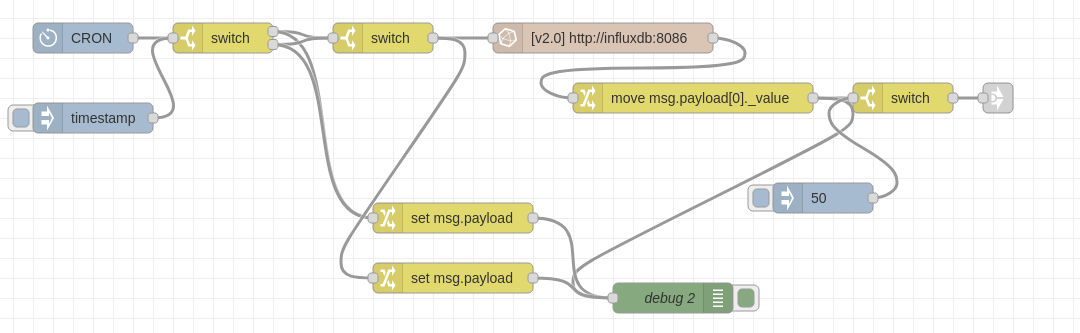
\includegraphics[width=\textwidth]{pump-activation.png}
  \caption{Überprüfungslogik für Pumpe in NodeRED}\label{fig:pump-activation}
\end{figure}

Abbildung \ref{fig:pump-activation} zeigt einen Screenshot der Überprüfungslogik für die Pumpe in NodeRED.
Das Programm wird jede Minute von dem CRON-Trigger gestartet und überprüft zunächst ob ein globales Flag gesetzt ist, welches die Überprüfung aussetzten würde.
Darauffolgend überprüft das Programm, ob für die nächsten 24 Stunden Niederschlag vorhergesagt ist.
Die Wetterdaten hierzu werden in einem Sub-Programm regelmäßig von der öffentlichen API des Deutschen Wetterdienstes geladen und in einer globalen Variable gespeichert.

Falls nicht, erfragt das Programm den durchschnittlichen Bodenfeuchtigkeitswert der letzten fünf Minuten von der InfluxDB.
Liegt dieser Wert unter 25\%, wird die Steuerungslogik für die Pumpe in einem Sub-Programm ausgeführt.
Dieses ist in Abbildung \ref{fig:pump-activation} dargestellt.

\begin{figure}[h]
  \centering
  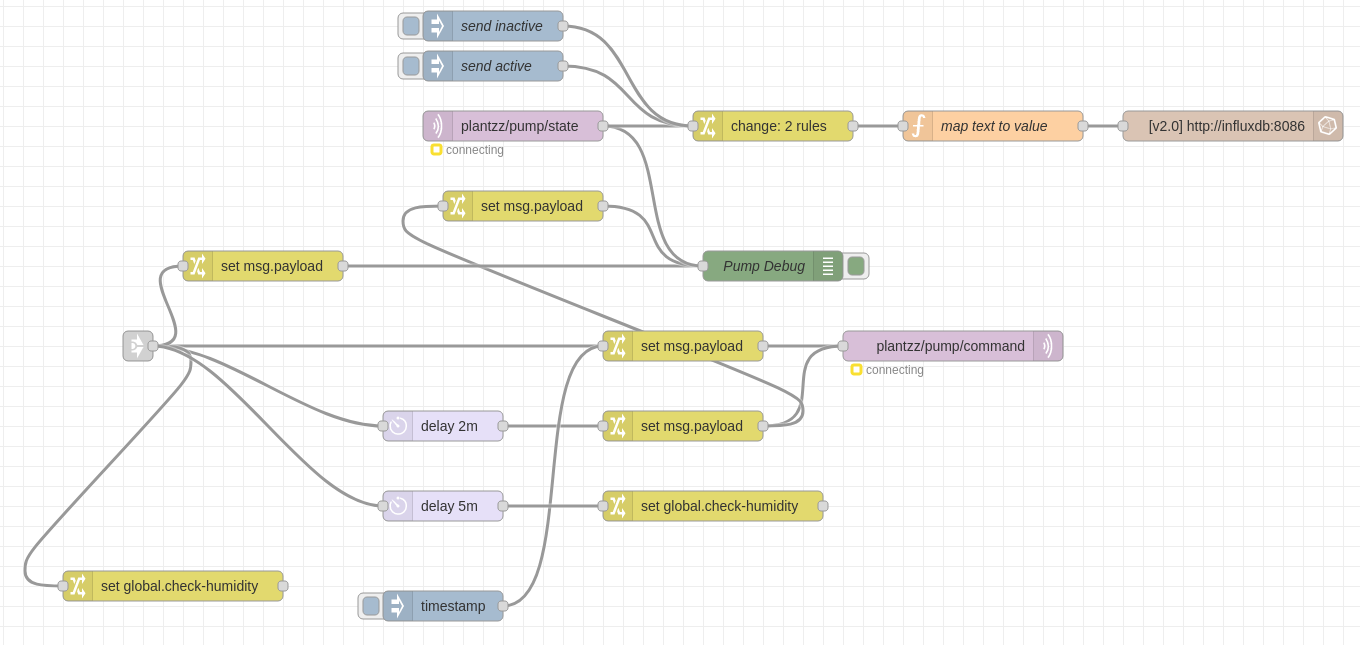
\includegraphics[width=\textwidth]{pump-control.png}
  \caption{Steuerungslogik für Pumpe in NodeRED}\label{fig:pump-activation}
\end{figure}

Beim Starten des Steuerungs-Programms wird unmittelbar eine Nachricht mit dem Aktivierungskommando an das MQTT-Topic der Pumpensteuerung versendet.
Zudem wird das globale Flag gesetzt, welches die die Überprüfungslogik deaktiviert.
Nach einer Verzögerung von zwei Minuten, wird das Deaktivierungskommando versendet und nach fünf Minuten wird das Flag zur Deaktivierung der Überprüfungslogik wieder zurückgesetzt.